\chapterimage{head2.png} % Chapter heading image
\chapter{Latex examples}

% ---------------------------------------------
% ---------------------------------------------
\section{Sample text}
This is sample paragraph extracted from bbc news.

Aerial footage showed lava from the Cumbre Vieja volcano spilling downhill and destroying several houses.

Mr Sanchez said authorities are closely monitoring fires that may start from the burning lava. The military and civil guard has been deployed to help.

The volcano last erupted 50 years ago.

It lies in the south of La Palma island, which is home to around 80,000 people.

The eruption started around 15:00 local time (14:00 GMT) and sent lava flowing down the hillside toward villages. 

This is text with some format. Some of the \textbf{greatest} discoveries in \underline{science} were made by \textbf{\textit{accident}}.

More usefull information about Latex is in: \url{https://www.overleaf.com/learn/latex/Creating_a_document_in_LaTeX}

% ---------------------------------------------
% ---------------------------------------------
\section{Itemizes and enumerates}
Itemize is a unordeder list made with points. Enumerate is a ordered list made with numbers.

Enumerate example:

\begin{enumerate}
\item First element
\item Second element
\item Third element
\end{enumerate}

Itemize example:

\begin{itemize}
  \item First element
  \item Second element
  \item Third element
  \end{itemize}

% ---------------------------------------------
% ---------------------------------------------
\section{Subsections}
OK, here is where I explain from where this is going to start, at that time I just had a micro-controllers and engineering design 
course my mind was set completely to find applicable theories and create useful things with them, which is the complete opposite of how astronomy works. 
First, there's no way to test an experiment with galaxies and most of the information is fuzzy and subjective (not all). 
The process of having an, let's say \emph{astronomy idea} is a result of applying all your physics knowledge and consider the \textbf{cosmological principle},

\subsection{Subsection example}
Since I found so much good information about pretty much everything I wanted to know about, I will just create a remark and let 
you know where you can find more specific information about, just like below.

\subsubsection{Subsubsection example}
Since I found so much good information about pretty much everything I wanted to know about, I will just create a remark 
and let you know where you can find more specific information about, just like below.

\subsubsection{Another subsubsection example}
Since I found so much good information about pretty much everything I wanted to know about, I will just create a remark 
and let you know where you can find more specific information about, just like below.

\subsection{Another subsection example}
Since I found so much good information about pretty much everything I wanted to know about, I will just create a remark 
and let you know where you can find more specific information about, just like below.

% ---------------------------------------------
% ---------------------------------------------
\section{References}
In \cite{book_key} and \cite{article_key} authors talk about bla bla bla.

% ---------------------------------------------
% ---------------------------------------------
\section{Images}
Figure \ref{fig:nine} shows bla bla. 

\begin{figure}[t]   % [t] means that the figure should be localed at the top (if it possible)
	\centering
    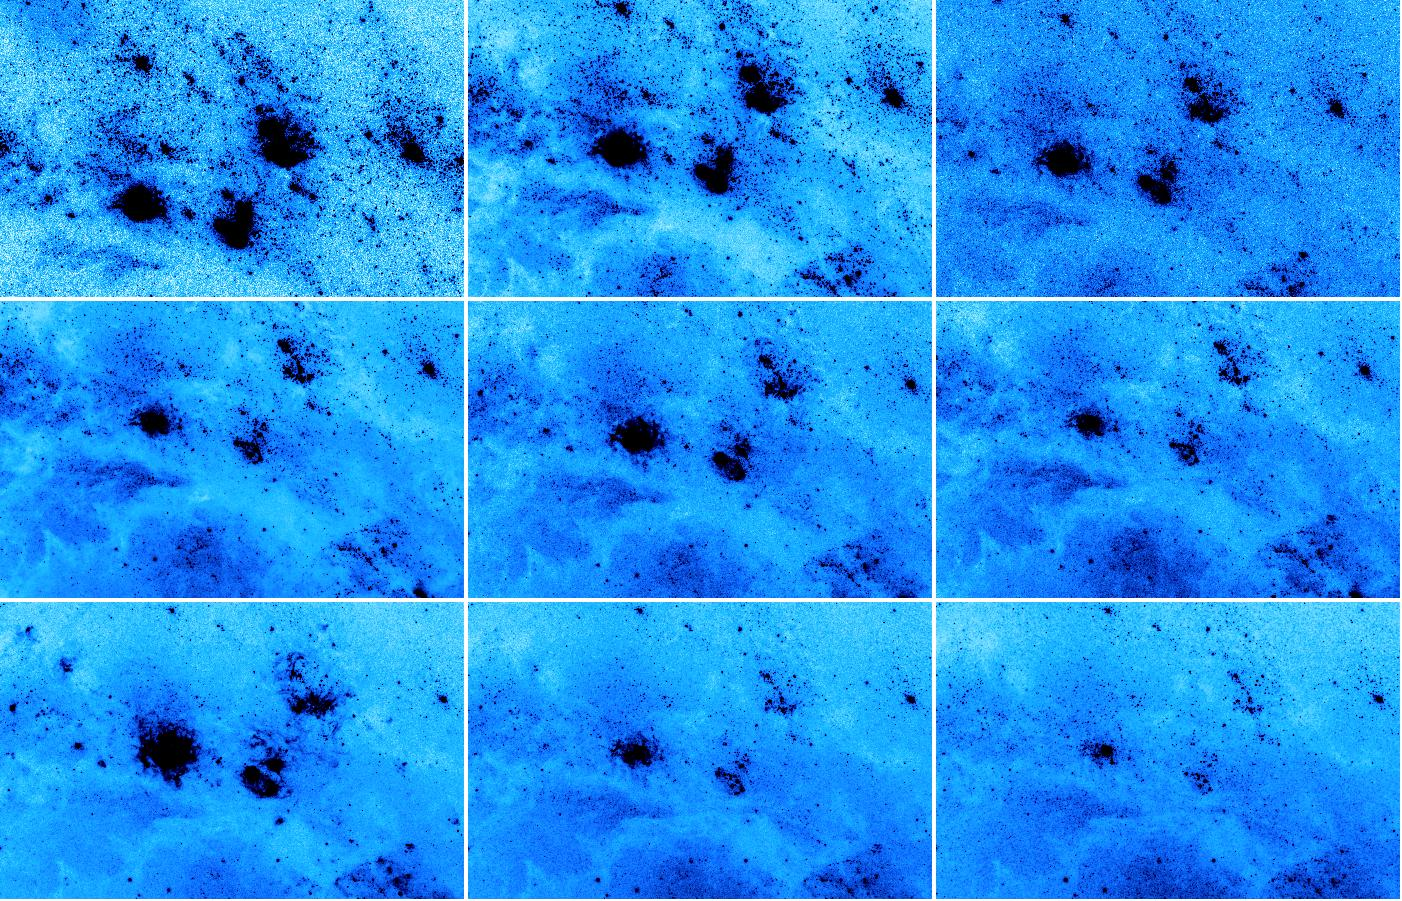
\includegraphics[width=0.87\textwidth]{nine.jpg}
    \caption{Example of how an object can look in 9 wavelengths}
    \label{fig:nine}
\end{figure}

% ---------------------------------------------
% ---------------------------------------------
\section{Tables}
Table \ref{tab:dos} shows bla bla bla.

\begin{table}[t]
    \centering
    \caption{WFC3/UVIS PSF FWHM informations for the selected dataset, as you can see the largest number here is 0.083 
    which means the poorest spatial resolution, this is the number used to calculate the convolution kernel, in order to 
    precess them all images must have the same spatial resolution.}
    \label{tab:dos}
      \begin{tabular}{ c c c }
      \hline\hline
      Filter / Config. & Central $\lambda$ & FWHM (arc sec)\\
      \hline
      F225W & 235.9 nm & $\sim$0.083\\      
      F336W & 335.5 nm & $\sim$0.075\\      
      F373N & 373.0 nm & $\sim$0.070\\
      F438W & 432.5 nm & $\sim$0.070\\
      F487N & 487.1 nm & $\sim$0.067\\
      F502N & 501.0 nm & $\sim$0.067\\
      F657N & 656.7 nm & $\sim$0.070\\
      F673N & 676.6 nm & $\sim$0.070\\
      F814W & 802.4 nm & $\sim$0.074\\    
      \hline
    \end{tabular}
  \end{table}
  

% ---------------------------------------------
% ---------------------------------------------
\section{Maths}
This an example of equation:

\begin{equation}
  \sum_{p\in [0,\ldots,n-1]} x[p] b^p
\end{equation}

